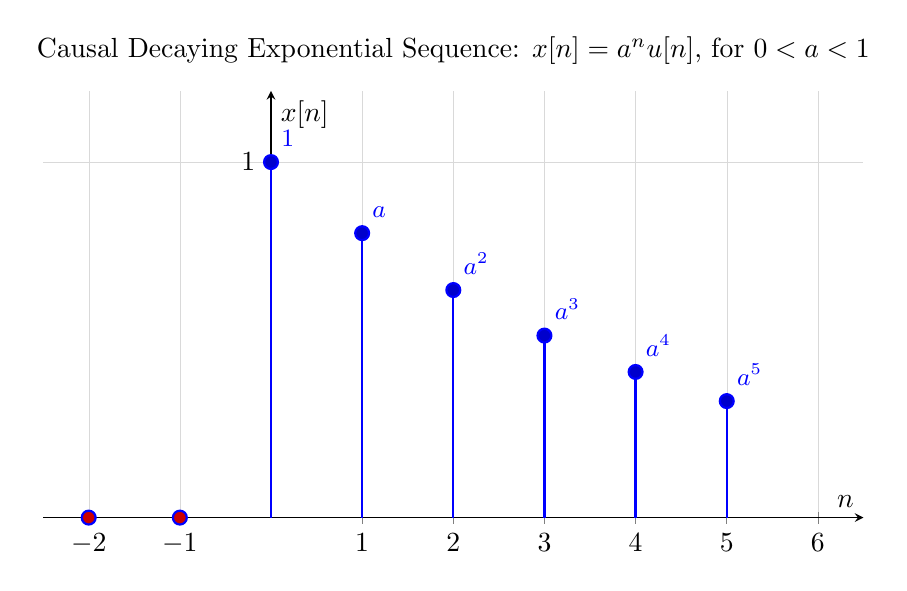
\begin{tikzpicture}
	% Define a style for our stem plots
	\pgfplotsset{
		impulse/.style={
			ycomb,
			blue,
			thick,
			mark=*,
			mark size=2.5pt,
		}
	}
	
	\begin{axis}[
		% Set the overall style
		width=12cm,
		height=7cm,
		% Title with the signal's definition and condition
		title={Causal Decaying Exponential Sequence: $x[n] = a^n u[n]$, for $0 < a < 1$},
		% Axis labels
		xlabel={$n$},
		ylabel={$x[n]$},
		% Position axes at the origin
		axis lines=middle,
		% Set axis limits
		xmin=-2.5, xmax=6.5,
		ymin=0, ymax=1.2,
		% Set ticks at key points
		xtick={-2, -1, 0, 1, 2, 3, 4, 5, 6},
		ytick={1},
		% Add a grid
		grid=major,
		grid style={line width=.1pt, draw=gray!30},
		]
		
		% Plot the non-zero impulses using a data table
		\addplot+[
		impulse,
		nodes near coords, % Add value labels from the 'label' column
		point meta=explicit symbolic, % Use the 'label' column for node text
		every node near coord/.style={
			anchor=south west, % Position labels
			font=\small,
			yshift=2pt,
		},
		] table [meta=label] {
			x   y        label
			0   1        {$1$}
			1   0.8      {$a$}
			2   0.64     {$a^2$}
			3   0.512    {$a^3$}
			4   0.4096   {$a^4$}
			5   0.32768  {$a^5$}
		};
		
		% Plot some zero-value points to show the effect of u[n]
		\addplot+[impulse] coordinates {
			(-2, 0)
			(-1, 0)
		};
		
	\end{axis}
\end{tikzpicture}